% !TEX root = ../thesis.tex

% Tutkimustuloksien merkitystä on aina syytä arvioida ja tarkastella
% kriittisesti. Tässä osassa on syytä myäs arvioida tutkimustulosten luotettavuutta.

% At this point, you will have some insightful thoughts on your implementation
% and you may have ideas on what could be done in the future. This chapter
% is a good place to discuss your thesis as a whole and to show your professor
% that you have really understood some non-trivial aspects of the methods you
% used. . .

\documentclass[thesis.tex]{subfiles}

\begin{document}

\chapter{Discussion}
\label{chapter:discussion}

This chapter begins with a discussion of the design decisions taken during the implementation of the application, and continues by presenting the findings made from the raw result data and Chapter \ref{chapter:results}. Last, challenges faced during the project and an outline for future research work are presented, and the research questions establised in Chapter \ref{chapter:research-questions} are reviewed. Motivation behind some of the design choices disussed in the earlier chapters are not reiterated here, and the interested reader is instead referred to Chapter \ref{chapter:design-implementation} and the related appendices \ref{appendix:camera-module} and \ref{appendix:capture-presets} for further information.

\section{Design Choices}

One of the early challenges in the project was to develop a smartphone-based method for capturing photoluminescence. A prototype of the camera module had already been developed prior the project for demonstration purposes. It provided good isolation from ambient light and even a built-in slot for different diffraction gratings and slits. However, the prototype required the taggants to be manually excited -- by toggling a UV flashlight by hand (Nightsearcher UV 365) -- as it did not have an integrated light source.

For product authentication purposes a more granular, programmatic control over the light source was required. Moreover, the added benefit of using a diffraction grating and a slit to achieve higher color resolution would have mostly been cancelled out by the loss of spatial information (taggant positioning) and its negative impact on the already weak Signal-to-noise ratio (due to the additional elements the photons would need to travel through). Furthermore, as the 3D printed mold of the early prototype -- used for attaching a smartphone to the module -- was designed only for Lumia 920, the integration of the Samsung S4 and Lumia 1020 would have increased the initial workload. Thus, an alternative, simple and more easily customizable cardboard prototype was implemented, as presented earlier in Chapter \ref{chapter:camera-module}. For comparison Figure \ref{figure:origina-camera-module} provides a wireframe of the original camera module prototype together with a sample image taken with a Lumia 920.

\begin{figure}[h!]
  \centering 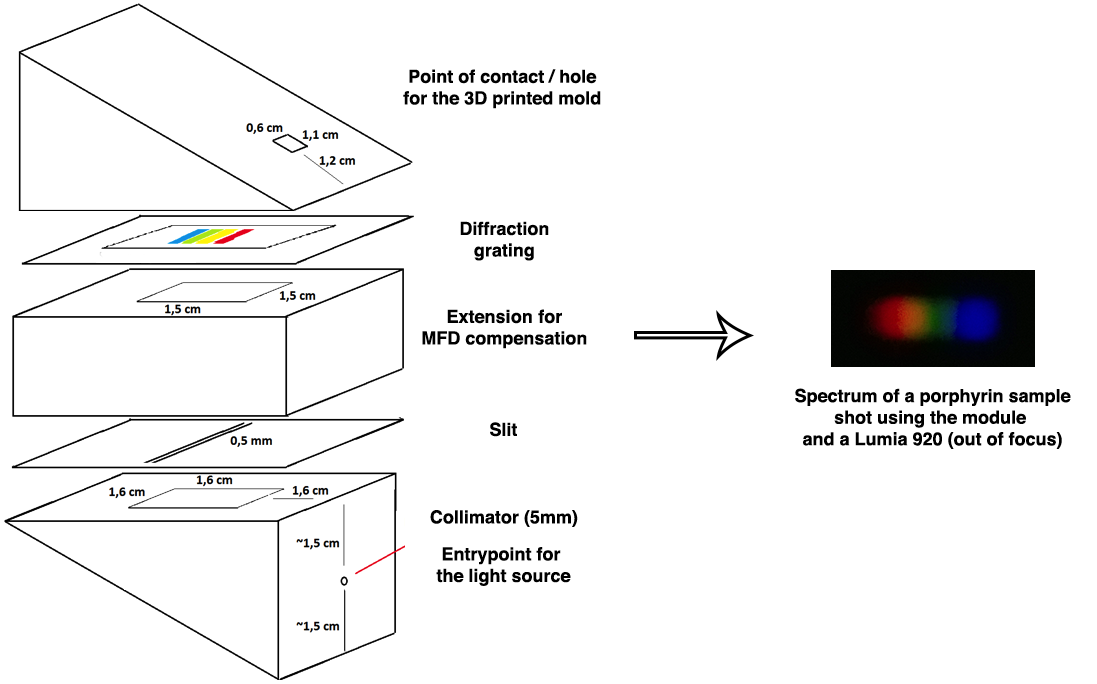
\includegraphics[page=1,width=\textwidth]{images/findings/original_camera_module}
  \caption{The design wireframe of the original camera module that included a diffraction grating and a slit. The 3D printed mold used for attaching a smartphone to the module was only designed to fit a Lumia 920.}
  \label{figure:origina-camera-module}
\end{figure}

The use of an external light source was required to normalize any differences in the light that smartphones emit. Moreover, the torch light in both the Samsung S4 and Lumia 1020 did not even emit the right kind of light (wavelength) to excite the taggants properly. The programmatic control of the light source required a connection to be established between the smartphone and the light source. Cross-modal communication by means of light signals proved to be a straightforward and adequate solution -- connecting the two devices via WiFi, Bluetooth or cable would have added unnecessary complexity both in hardware and software.

As one of the goals of the project was to be able to compare results across different smartphones (as per \ref{R1}), the capture parameters needed to be standardized. For this purpose a set of capture presets were defined (see Table \ref{table:capture-presets}). The preset values for the \emph{interval} duration were configured based on the taggants. As described in \cite{luminova}, the Luminova\textregistered\ pigments are fairly slow (long emission duration). For the smartphone to be able to capture any significant change in the emission also the capture intervals needed to be long. The appropriate intervals of 200, 400 and 600ms were eventually derived empirically. The preset resolutions were set to the highest preview frame resolution supported by the given platform. As Windows Phone 8.1 did not support preview resolutions higher than $1280\times720$px only three presets were defined for the Lumia 1020.

Different focus strategies were applied depending on the platform. Android 4.4.2 (API level 19) does not support setting focus to a fixed minimum distance. Therefore, macro focus mode was used to guarantee the Samsung S4 could still acquire accurate focus around its MFD. The macro focus mode however required the use of the focus light. The torch light was therefore not used on the Samsung S4 to avoid triggering the light source twice -- the focus light would function as the trigger instead. Unfortunately, the focus light of the S4 introduced some bias to the pipeline as it contained enough energy to excite a few of the taggants as shown on the left in Figure \ref{figure:artefacts}. On the Lumia 1020 the focus was set to a fixed minimum distance (MFD), and the torch light was used as the light source trigger.

A number of camera parameters were set to a fixed value as shown in Table \ref{table:capture-presets-fixed}. The number of frames (samples) to capture per fingerprint was fixed at five frames. It was empirically observed that additional frames would not provide much data due to decreasing SNR. Furthermore, capturing more frames would have led to worse experience for the user as the capture and processing times would have gotten longer. Capturing three or four frames could have provided similar results, but as emission peaks were still observed in some of the taggants even after 3000ms, the frame count was not adjusted any lower. Moreover, it would be trivial to retroactively compute results based on four or less frames if necessary.

The camera white balance was set to the \emph{Daylight} preset value as Android 4.4.2 does not support manual white balance adjustment. The Daylight preset was chosen over other available white balance presets as it typically applies the least compensation and corresponded well with the color temperature (5600K) of the experiment light source (Yongnuo YN565EX). The Daylight preset represents roughly a temperature of 5500-6500K depending on the vendor.

Other capture parameters set to a fixed value were \emph{delay} and \emph{ISO}. Delay -- the time to delay the capture of the first frame (after the light source has been triggered) -- was determined empirically by observing when the focus light of the Samsung S4 would no longer introduce capture artefacts. An example of the artefact caused by the interference from the S4's focus light is presented Figure \ref{figure:artefacts} in the middle. The interference was believed to have been caused by the smartphone's decaying LED light interfering with the preview feed signal. The Lumia 1020 exhibited no such behaviour.

The capture ISO was set to \emph{auto} as Samsung S4 was unable to lock exposure for the time of the capture when a manual ISO value was used. This was believed to be a bug in the camera API of Android 4.4.2 when frames are captured via the preview feed. Ideally, a low ISO value of ISO100 would have been used to avoid introducing any unwanted noise to the pipeline.

The motivation for using hue and hue-saturation histogram analysis as the basis of the fingerprint matching was largely inspired by how luminophores are studied in chemistry by means of spectroscopy. The idea of the histograms was to provide a rough estimate of the ``emission spectrum'' (color distribution) of the taggant. The capture of a proper emission spectrum would have required a way diffracting the incident light (e.g. via a diffraction grating) and the application of proper color calibration for translating RGB values into wavelengths. The parameter values supplied to the fingerprint and histogram methods for analyzing the captured data were largely based on trial and error, that is, on apriori assumptions and observations on how the results behaved when a given parameter was adjusted.

Binary thresholding was used as the primary filter due to its simplicity and fit for the context. As the frames consisted of small color blobs on a dark background the dark pixels on the background could be easily filtered by a binary thresholding level of 15\%. The hue bin size was set to 180, which is also the maximum number of hue bins OpenCV supports (for 8-bit images). Internally OpenCV's \emph{calcHist()} function encodes the hue values from 360 down to 180 for better performance. A bin count of 60 was used for saturation as it was assumed that smaller saturation bin sizes would increase computation time of histogram method while having no significant impact on the final similarity score.

The persistance threshold used by the fingerprint method for peak selection was set to 20\% purely based on which threshold seemed to provide neither too many nor too few peaks. The implications of this naive approach are briefly discussed in Chapter \ref{chapter:findings}. The penalty weight, damping coefficient and delta threshold of the fingerprint method were also derived empirically by first assigning them logical initial values and adjusting those until the results of randomly selected samples of the data seemed to improve.

While the tracing process was built to be storage backend agnostic, a NoSQL database solution was selected over a relative DBMS technology due to the better schema flexibility of NoSQL databases. Furthermore, a document-based NoSQL DBMS is ideal for storing JSON data like the fingerprint documents (Appendix \ref{appendix:fingerprint}). A flexible schema also allows changing document fields without costly migrations, which speeds up the development cycle (imperative for new projects) and helps in including unstructured metadata to documents (e.g. vendor specific fields). CouchDB was chosen as the underlying NoSQL implementation for its wide adoptance and support for client-side data replication (through PouchDB).

The original corpus included taggant \emph{V}, but as it was suspectible to overexposure artefacts -- due to a human error in the taggant preparation process -- as seen in the image on the right in Figure \ref{figure:artefacts} it was omitted from the final corpus.

\section{Findings}
\label{chapter:findings}

Based on Figure \ref{figure:taggants} it is apparent that the shape and size of sibling fingerprints vary. This is due to the fact that luminophore was pipeted on the cartons by hand in an uncontrolled environment. Another side effect of the manual taggant creation process can be seen in the non-uniform luminophore concentration of taggant \emph{13SVb} -- the highly concentrated areas of the taggant have been overexposed. The relative size difference between the taggants captured with the Samsung S4 and Lumia 1020 is due to the difference in the lens MFD (10cm and 15cm, respectively).

Figure \ref{figure:taggants} also shows that taggant \emph{S} is hardly visible (its visibility in the figure has been improved for demonstration purposes). This could be due to the light source not emitting the appropriate wavelength for exciting the taggant, or the sensor's low sensitivity to the blue pigment (\emph{DB} in Appendix \ref{appendix:taggants}). Differences in the visibility of the taggant between the Samsung S4 and Lumia 1020 indicates the latter. The poor sensibility of the blue pigment is also seen in the visual similarity of the \emph{13SP} and \emph{P} taggants. Based on these discrepancies alone it is obvious that taggants captured by the Samsung S4 and Lumia 1020 can not be unambiguously compared with one another.

The fingerprint clusters visualized in Figure \ref{figure:clusters} suggest that histogram method outperforms the fingerprint method. It is able to find 50\% more clusters in the corpus as well as cover over 95\% (137/144) of all the fingerprints (vs. 66,67\% of the fingerprint method). Furthermore, the clusters are of better ``quality'' as there are several groups of 2-4 sibling fingerprints -- clusters that have similar size and color. Based on the results of the clustering taggants \emph{24VP} and \emph{24SP} perform the best while \emph{13SV} and \emph{24SV} provide mixed results.

Figure \ref{figure:tags_presets} provides more insight into the performance of individual taggants and presets. Unsurprisingly, long intervals help distinguish the taggants better, although no significant change in the performance between presets of 200ms and 400ms interval can be observed. The Windows Phone presets (\emph{wp}) fare better, which is expected due to the higher quality camera in the Lumia 1020. The relatively poor performance of taggant \emph{13SV} can be attributed to the overexposure artefact in its \emph{b} sample and the fact that it noticeably differs from its sibling sample as depicted in Figure \ref{figure:13SV}. In the case of taggant \emph{S} on the other hand, the drop in the number of matches can be attributed to the poor detectability of the blue pigment causing relatively low SNR. Somewhat surprising, however, is how relatively few times taggant \emph{13SP} is matched by the histogram method in comparison to taggant \emph{P}. The raw result data shows that a good number of \emph{13SP} based fingerprints (8) actually match closer to taggant \emph{P} than their siblings. Seems as if the blue pigment has no effect on the emission as further evidenced by the visual similarity of \emph{13SP} and \emph{P} in Figure \ref{figure:taggants}.

\begin{figure}[h!]
  \centering 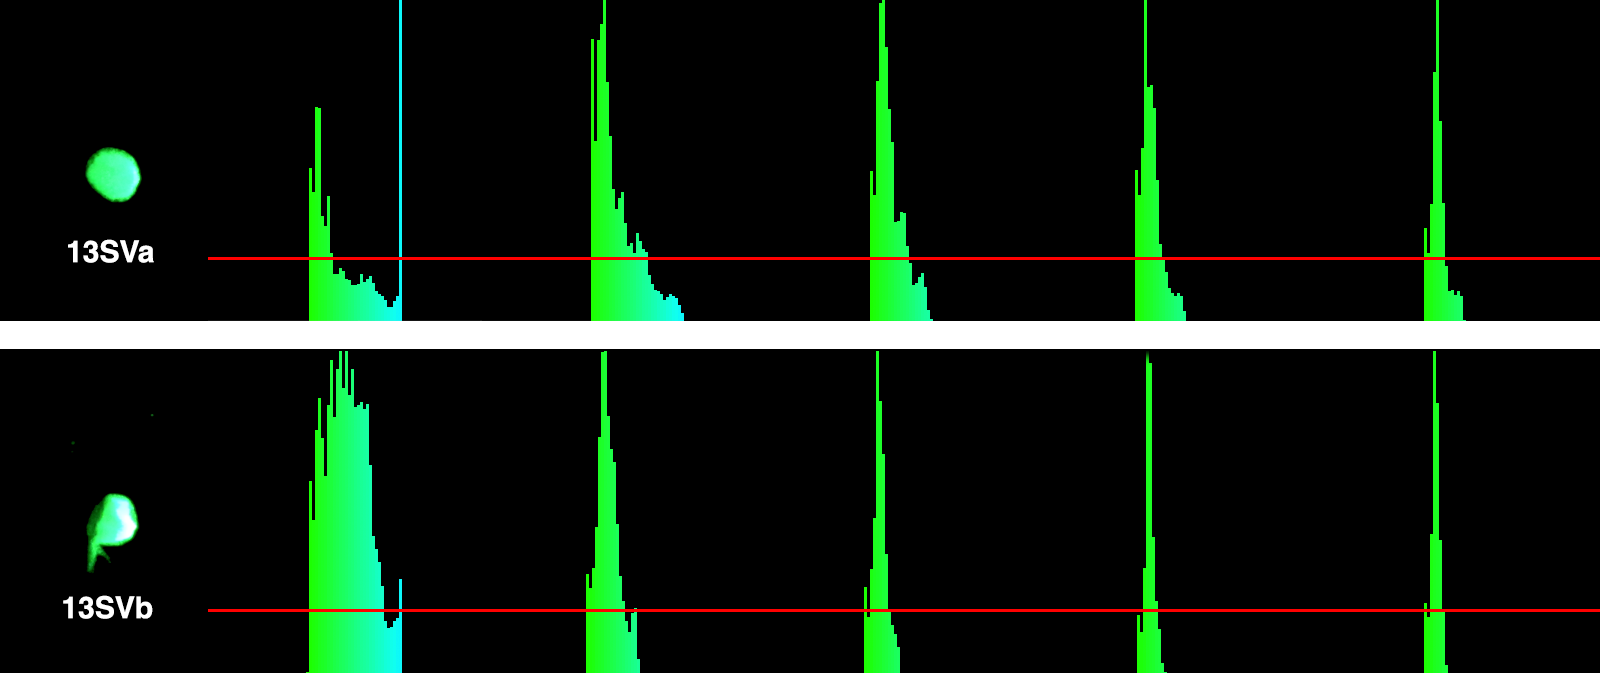
\includegraphics[page=1,width=\textwidth]{images/findings/13SV}
  \caption{Due to an artefact introduced during taggant preparation the first two samples of taggant \emph{13SVb} are largely dissimiliar compared to its sibling \emph{13SVa}. The red horizontal line depicts the persistance threshold.}
  \label{figure:13SV}
\end{figure}

Based on Figure \ref{figure:tags_presets} increasing the $B_{count}$ boundary from three to six fingerprints seems to have minimal effect on the number of matches found. The success rate and precision curves given in Figures \ref{figure:match_precision_fingerprint} and \ref{figure:match_precision_histogram} support this observation: after a certain level of $B_{margin}$ the success rate stagnates regardless of the $B_{count}$, while precision continues to decrease. Moreover, a combination of high $B_{count}$ and $B_{margin}$ degrades user experience as a larger number of matches would be found resulting in more products to be retrived for the user to choose from. An ideal combination of $B_{margin}$ and $B_{count}$ seems to range from 50-80\% and 3-6 for the fingerprint method, and from 20-40\% and 3-8 for the histogram method. If anything, excessively increasing $B_{margin}$ will only lead to more false positives for the user to filter. On the other hand, as seen in Table \ref{table:match_precision_count1}, if only the best match ($B_{count} = 1$) was processed, the user would be displayed the correct product in less than 50\% of the time, regardless of the method.

As indicated by the clustering in Figure \ref{figure:clusters} and the match distributions in Figure \ref{figure:tags_presets} taggants \emph{24VP} and \emph{24SP} provide good results, especially with presets of the 600ms interval. The higher pigment concentrations of \emph{24VP} and \emph{24SP} seem to improve the SNR. Using the histogram method with boundary conditions of $B_{count} = 4$ and $B_{margin} = 30\%$ the success rate/precision of \emph{24SP} is 100\%/84,26\%, and 94,44\%/57,35\% for \emph{24VP}, respectively.

Given the above it is surprising that the performance of \emph{24SV} -- using the same method and boundary conditions as above -- is significantly worse (success rate: 55\%, precision: 46\%). The raw data shows that \emph{24SV} actually comes very close to matching its siblings. In 16 out of the 18 tracings (9 presets $\times$ samples \emph{a} and \emph{b}) 50-100\% of the matches were of the correct taggant (\emph{24SV}). Thus, the low the success rate of \emph{24SV} was largely due to the (histogram) method's inability to distinguish between presets. The higher concentration -- the addition of $50\mu l$ of green and blue pigments (\emph{G} and \emph{DB}) -- did not indeed produce any significant change in the emission as illustrated by Figure \ref{figure:SV}. The taggant \emph{24SV} appears to attenuate too \emph{slowly} for the camera sensor to capture any change. In general both methods were better at distinguishing the fingerprints by taggant than by preset as shown in Table \ref{table:match_precision_count1}.

\begin{figure}[h!]
  \centering 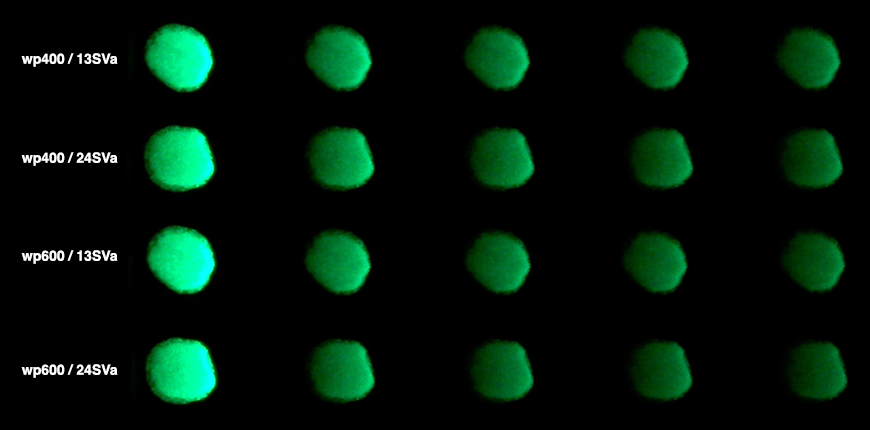
\includegraphics[page=1,width=\textwidth]{images/findings/SV}
  \caption{Regardless of the increase in luminophore concentration and capture interval duration from 400ms to 600ms no significant changes could be observed between taggants \emph{13SV} and \emph{24SV}.}
  \label{figure:SV}
\end{figure}

Overall the histogram method performs better than the fingerprint method. The fingerprint method provides a success rate of approximately 65\% at best, while the success rate of the histogram method ranges up to 95\%. Interestingly enough these success rates are already indicated by Figure \ref{figure:clusters} in how many fingerprints the clusters cover (137 vs. 96 out of 144). Perhaps one equally descriptive metric of the performance of the two methods is the ratio of misses, which is twice as high when using the fingerprint method with $B_{count} = 1$ as shown in Table \ref{table:match_precision_count1}. Based on the standard deviation and mean of $B_{margin}$ visualized in Figure \ref{figure:match_precision_margin} the histogram method is also better at separating (distinguishing) the fingerprints from one another: for the histogram method the margin (y-axis) -- within which the matches fit -- is higher (up until $B_{margin} \approx 85\%$). The tradeoff of the more accurate histogram method is the increase in required computation time, storage space and bandwidth.

The most significant pitfall of the fingerprint method is the static nature of its analysis parameters. Figure \ref{figure:fingerprint-method-pitfalls} illustrates two example cases where this causes problems. The raw result data revealed that fingerprint \emph{wp\_600/13VPb} matched the rest of the corpus poorly when compared using the fingerprint method. This was due to the excessive number of peaks found in its fourth sample, which in turn resulted in relatively high $P_{hue}$ and $P_{int}$ scores. A fixed persistance threshold -- depicted by the red line in Figure \ref{figure:fingerprint-method-pitfalls} -- works poorly when SNR is low as shown by the plot on the left. Moreover, using a fixed threshold the fingerprint method was unable to account for slight variations in the hue distribution caused by e.g. residual afterglow from a previous capture as seen in Figure \ref{figure:fingerprint-method-pitfalls} on the right.

\begin{figure}[h!]
  \centering 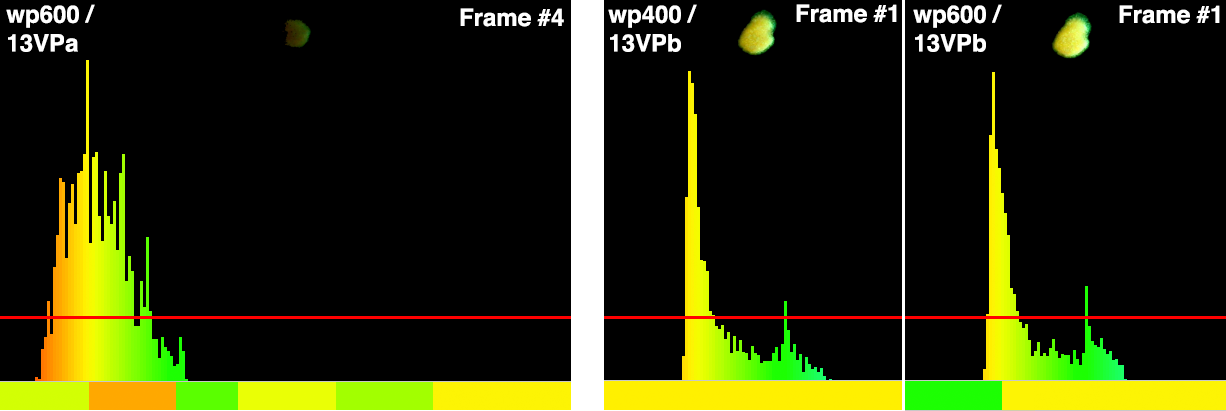
\includegraphics[page=1,width=\textwidth]{images/findings/persistance_pitfall}
  \vspace{-8mm}
  \caption{A fixed persistance threshold (red line) provided inaccurate results when SNR was low (left plot). Moreover, a fixed persistance threshold was unable to account for slight variations in the hue distribution -- caused by e.g. residual afterglow from a previous capture -- leading to inconsistent results (right plot). The color bars along the x-axis depict the relative amounts of different hues in the histogram.}
  \label{figure:fingerprint-method-pitfalls}
\end{figure}

Increasing hue bin size based on SNR or improving SNR itself by using a more novel filtering technique could help address these issues. Outstanding challenges and prospects for future work are discussed further in the next chapter. Based on the results presented in Chapter \ref{chapter:results} and the findings above the following is concluded:

\begin{enumerate}
  \item The histogram method performs better overall, but the fingerprint method allows stricter space and time requirements
    \begin{itemize}
      \item proposed fingerprint method $B_{margin}$ and $B_{count}$: 50-80\% and 3-6
      \item proposed histogram method $B_{margin}$ and $B_{count}$: 20-40\% and 3-8
      \item boundary conditions could be adjusted dynamically as per user feedback (e.g. implementing a \emph{Show more} functionality)
    \end{itemize}
  \item Longer intervals provide better results, but have implications for user experience and depend largely on the taggant's excitation lifetime
  \item Lumia 1020 outperforms the Samsung S4 due to its better quality (less noisy) sensor and the artefacts inherent in the Samsung S4
  \item Taggant preparation has a significant impact on fingerprint tracing
    \begin{itemize}
      \item sibling taggant shape, size and concentration should be identical
      \item the luminophore should be fast enough for any significant change to be detected (preferably an excitation lifetime of \textless\ 5000ms)
      \item the wavelength of the light source should match the excitation wavelength of the luminophore for proper photoexcitation
    \end{itemize}
  \item Novel filtering techniques and dynamic persistance threshold (e.g. based on SNR) would likely improve the performance of the fingerprint method.
\end{enumerate}

\section{Challenges and Future Work}

The primary challenge in systems that rely on color information -- be it an image of a taggant or its emission spectrum -- is color calibration. As RGB is a device-dependent color model, different smartphones detect and reproduce a given RGB value differently: the sensor's response to the individual R, G, and B levels vary from vendor to vendor -- or even in the same device over time due to e.g. fabrication and aperture variations. Thus, an RGB value does not define the same color across devices without some kind of color management process.

There are mainly two modules responsible for the color management (color correction) of a digital instrument: illuminant estimation (capture context) and color matrix transformation (color profile), the purpose of which is to transform the sensor output to a standard (rendered) color space. In this work the capture context could be made constant by using the same camera module (and the associated light source). Color profiles would however need to be created separately for each supported smartphone model. And, since a color profile is only really useful when it is applied on \emph{unrendered} sensor data, the image would need to be captured in RAW format. Thus, proper color calibration would have implications for both scalability (maintenance of color profiles) and performance (RAW image capture). \cite{multiple_cameras} \cite{color_correction_pipeline}

Perhaps a more practical approach would be to omit color calibration altogether, and instead, have one fingerprint database per each smartphone model. This would offload the complexity of the \emph{normalization} to the storage layer where each database would contain the fingerprint corpus for a given smartphone model. The impact on scalability would also be minimal as NoSQL databases are \emph{horizontally scalable} \cite{nosql_scalability}.

Due to the lack of support for burst mode and timed capture by the camera API of both Android 4.4.2 and Windows Phone 8.1 images needed to be captured using the preview frame feed. This was unideal for two reasons. First, the preview feed degrades image quality for better FPS. Second, the application logic required for implementing the capture of the image data from the preview feed incurred additional complexity. Furthermore, in the case of Android, artefacts were introduced. As smartphone camera APIs continue to mature, new capture methods like burst mode will hopefully provide a more stable and higher quality approach to scheduling the capture of multiple frames. In the interim, the use of high definition video remains an intriguing -- although perhaps equally challenging -- alternative.

The accuracy of the fingerprint tracing could also be improved by applying additional selection criterion, such as structural and spatial similarity. For example, in a similar way to CryptoGlyph\textregistered\ taggants of various shapes and sizes could be used to form discrete patterns to allow fingerprints to be compared in one additional dimension.

Regardless of the prospect of corpus normalization techniques (color calibration), more robust capture functionality (native burst capture) or additional selection semantics (spatial dimension) the methods presented in this thesis for analyzing and matching fingerprints can still remain applicable for small scale, internal authentication needs. As realised in the previous chapter, the histogram method should be the preferred method for matching fingerprints. The fingerprint method could prove useful as a lightweight \emph{fingerprint descriptor} for querying and filtering larger sets of fingerprints. However, for better robustness its apparent pitfalls -- as outlined in Chapter \ref{chapter:findings} -- would need to be addressed first.

Equally relevant to that of the capture and analysis methods are the luminous properties of the taggants and the light source. The LumiNova\textregistered\ pigments used in the experiments -- originally developed for use in watch dials -- were not entirely ideal test subjects. Their relatively long excitation lifetime made them difficult to differentiate. Ideally, the full-spectrum white light source used for the photoexcitation would also have been replaced by a less powerful light source of a specific wavelength range for a more controlled and realistic experimentation setting. The light source should be small to be practical but also powerful enough to excite the taggant. A light source emitting a specific wavelength range would likely be better than a general purpose full-spectrum white light. However, as different luminophores have slightly different excitation wavelength ranges, the question becomes which wavelength range the light source should cover?

The robustness of the luminophores poses another challenge as luminophores are subject to \emph{photobleaching} (or fading): after many absorption-emission cycles the underlying molecules begin to deteriorate leading to alterations in the luminescence. The loss of activity caused by photobleaching can be controlled by reducing the intensity or time-span of light exposure, by increasing luminophore concentration, by reducing the intensity (frequency) of the light source, or by employing more robust luminophores that are less prone to bleaching. The robustness as well as excitation wavelength and lifetime of a luminophore can be artifically tailored for the application. However, this has implications for cost-effectiveness as artificial fabrication of luminophores is often a tedious and costly process.

On the application side, the outstanding challenges relate to offline support and security. Client-side storage limits vary by browser and depend on the device's disk quota policies \cite{mobile-browser-quota}. Therefore predicting the available storage space and managing large amounts of data using browser storage APIs can prove difficult. Especially in the case of the preferred, but storage space heavier, histogram method the persistance logic would need to be migrated from the browser into native code for proper offline support. The migration of the existing persistance logic (PouchDB) would however be fairly straighforward using the SQLite plugin for Apache Cordova\footnote{\url{https://github.com/nolanlawson/cordova-plugin-sqlite-2}}.

For improved application security any vulnerable business logic running within the web view (JavaScript code) would need to be re-implemented in the platform native language or C/C++. For example, the fingerprint matching algorithm used by the fingerprint method, and run in the web view, could easily be reverse engineered by inspecting the source code via e.g. Google Chrome's Web Developer Tools -- even minified and mangled JavaScript would be a mere impediment for a diligent hacker to decipher. Alternatively, all sensitive information (fingerprint data and the related algorithms) could be hosted on the server only. The tradeoff would however be the loss of offline support and longer latency (transfer of captured frames to the server) for improved security and simpler architecture.

Possible attack scenarios include MitM attacks or getting physical access to the device. The fingerprint metadata database (as presented in Table \ref{table:fingerprint-metadata-schema}) works as a layer of indirection by allowing the fingerprint data stored on the device to be linked to products without exposing (locally storing) any potentially vulnerable information (e.g. \emph{cid} and \emph{tid}) to the attacker. Even when connected to a suspectible network a conscious user could fallback to offline behaviour to ensure that the product authentication response could not be tampered with by a malicious third party in control of the network. Physical attacks against the local database could be guarded against e.g. by periodically computing and validating a hash of the local database against a remote copy to check for any data corruptions.

The current authentication logic of using a predefined username and password stored in the application should be extended to a proper user authentication by enforcing user account creation. While the traditional cookie-based authentication scheme used by the DBMS (CouchDB) can be vulnerable to CSRF attacks, no CSRF attacks vectors currently exist as all the required public endpoints of both the DBMS and the application server are HTTP GET (read-only). The default, cookie-based authentication layer of the DBMS could however be replaced by modern token-based authentication such as JSON Web Tokens (JWT) for improved scalability. And, as for platform support, the WebView app architecture would allow extending support for iOS with minimal effort. Moreover, less platform-specific code would need to be written for iOS, as its APIs can be directly invoked from C++ -- as opposed to on Android and Windows Phone, for which JNI and C++/CX bridging is required as referred to previously in Chapter \ref{chapter:taggant-analysis}.

\clearpage
\section{Review of Research Questions}

\begin{itemize}[label=, leftmargin=*]
  \item \textbf{RQ1}: How can photoluminescence and smartphones be integrated for product authentication purposes?\\\\
  To induce photoluminescence a proper light source is required. Fabrication of luminophores to match the flash/torch light emission spectrums of various smartphones does not scale and therefore an external light source is a necessity. Synchronization of the external light source and the smartphone can be achieved via existing technologies such as WiFi or Bluetooth, or \emph{cross-modally} as done in this work. Regardless of the communication technique, a communication interface (e.g a WiFi receiver or a light sensor) will need to be integrated into the external light source. Furthermore, to physically align the light source with a given smartphone's camera, smartphone model specific adapters are required. Ideally, the photoluminescent material (luminophores) would only react to light from the light source so that no additional gadgets would be required to isolate it from ambient light. Once a proper light source and luminophores tailored for it are developed, the application developer can focus on leveraging the sensor RGB data to meet the desired product authentication needs.

  \item \textbf{RQ2}: Which factors affect the analysis of photoluminescent material (luminophores) in the context of smartphones?\\\\
  The camera lens, sensor and supported capture formats have the biggest impact on luminophore analysis. The closer the luminophore can be captured without image blur, the better, as more pixels are allocated for recording the photoluminescence. This proximity is dictated by the lens MFD, which depends on how the lens (lens array) of the given smartphone is constructed. The sensor's interpretation of the RGB signal varies from vendor to vendor so matching luminophore \emph{fingerprints} against an output produced by another capture device is redundant without proper color calibration (normalization). However, color calibration introduces a host of problems in itself (color profile creation, RAW processing), and thus, a more practical approach would be to compare the output against samples captured with the same device. This approach has implications for scalability however as it requires apriori storage of luminophore samples for \emph{each} supported smartphone model. Support of higher capture resolution and unrendered image formats are likely to provide more accurate results with the cost of increased computation time and space.

  \item \textbf{RQ3}: Does modern smartphone technology provide the means for photoluminescence based product authentication in practice?\\\\
  Photoluminescence can be utilized by current smartphone technology for product authentication needs, but only at small scale and in a controlled (internal) environment. The most sigificant impediment for wider adoption is the need for an external light source and the challenges of tailoring luminophores cost-effectively. The luminophores need to have a good resistance against photobleaching and a narrow excitation wavelength matching the emission wavelength of the light source. The emergence of modular smartphone technology as evidenced by the early Sony QX product line, the recently released LG G5 and the upcoming Google Ara smartphones hold promise for native integration of different 3rd party modules (such as the external light source) in the future.
\end{itemize}

\end{document}